% \section{Towards System 2 RAG \todo{revisit section name}}
\section{Design components}
\label{sec:sys2}
%todo 



To achieve effective System 2 RAG pipelines, it is essential to address challenges in both data and model aspects. System 2 decision-making relies on an organized, contextually rich data pool for informed outcomes, making efficient identification and organization of relevant information critical. Data enhancements, such as data discovery agents, play a key role by locating, structuring, and tagging pertinent data to create a streamlined and accessible knowledge base. Similarly, selecting and configuring models for each task is crucial. Choosing the right model, tuning it to align with user expectations, and ensuring seamless integration with the data pipeline all contribute to achieving optimal performance. 
In this section, we provide a high-level overview of our work in tackling these data and model challenges in developing a System 2 RAG pipeline.
\subsection{Data-level enhancements}


\subsubsection{Data Discovery}
As an initial effort to understand the potential impact in the data discovery task, we adapted existing datasets and benchmarks in open-domain --- from question answering and complex reasoning tasks to natural language querying over structured data --- to evaluate coarse- and fine-grained data discovery and task execution performance. Our experiments reveal the impact of data retriever design on downstream task 
  performance --- $46\%$ drop in task accuracy on average ---
  across various modalities, data sources, and task difficulty. The results indicate the need to develop optimization strategies to identify appropriate LLM agents and retrievers for efficient execution of CASs over enterprise data. This need is well-aligned with the System 2 type of thinking, in which before performing the retrieval, there is a need for reasoning on what data is available and how it should be retrieved. After such a reasoning step, the retrieval (and the RAG results in general) have the potential to improve.

 

\begin{figure}[!htb]
    \centering
    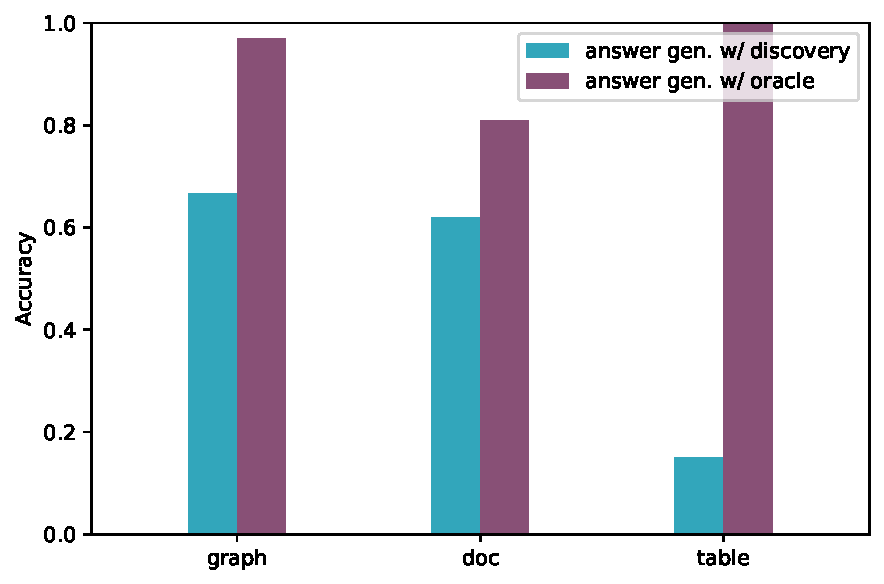
\includegraphics[width=0.5\linewidth]{submissions/Estevam2024/figures/answer_gen.pdf}
    \caption{Task execution performance degrades due to poor data discovery despite the purported proficiency of LLMs. }
    \label{fig:answer_gen}
    \vspace{-10pt}
\end{figure}

When we explored the impact of data discovery performance on the accuracy of downstream task execution. Figure~\ref{fig:answer_gen} captures the task execution accuracy for two scenarios: oracle and discovery. Oracle is the case where the ground truth discoverable element is provided to the LLM (\eg GPT-3.5 turbo) to provide the final answer to a question. Discovery captures the scenario where elements retrieved by the best-performing document, sub-graph, and table discovery models are provided to the LLM. We observe a significant drop in performance from \emph{oracle} to the \emph{discovery} scenario,  showcasing a $46\%$ decrease in accuracy.

\subsubsection{Less is More for Evaluation}


Evaluating text generation is crucial for creating high-quality systems. However, aligning automatic evaluation metrics with human judgment remains challenging~\cite{bhandari-etal-2020-evaluating,fabbri2021summeval}. While LLMs demonst
rate promising correlations with human evaluations, they encounter issues like high costs and the Lost-in-the-Middle problem~\cite{liu2023lost}, where key information in the middle of lengthy documents is frequently overlooked in summary evaluations.

To tackle these challenges, \cite{wu2024less} introduced a straightforward yet effective approach known as \textit{Extract-then-Evaluate}. At run-time, this method begins by extracting significant sentences from a lengthy source document and concatenating them until the extracted text reaches a predefined length. Subsequently, it assesses the quality of the summary based on this extracted content using LLMs. Figure ~\ref{fig:less_is_more} shows the overview of our approach. Notice that \emph{Extract-then-Evaluate} brings a System 2 type of thinking. The evaluation requires the analysis of the original document and the identification of the key elements. Only after reasoning and identifying such key elements is the evaluation of the quality of the summary performed.

\begin{figure}[!t]
  \centering
  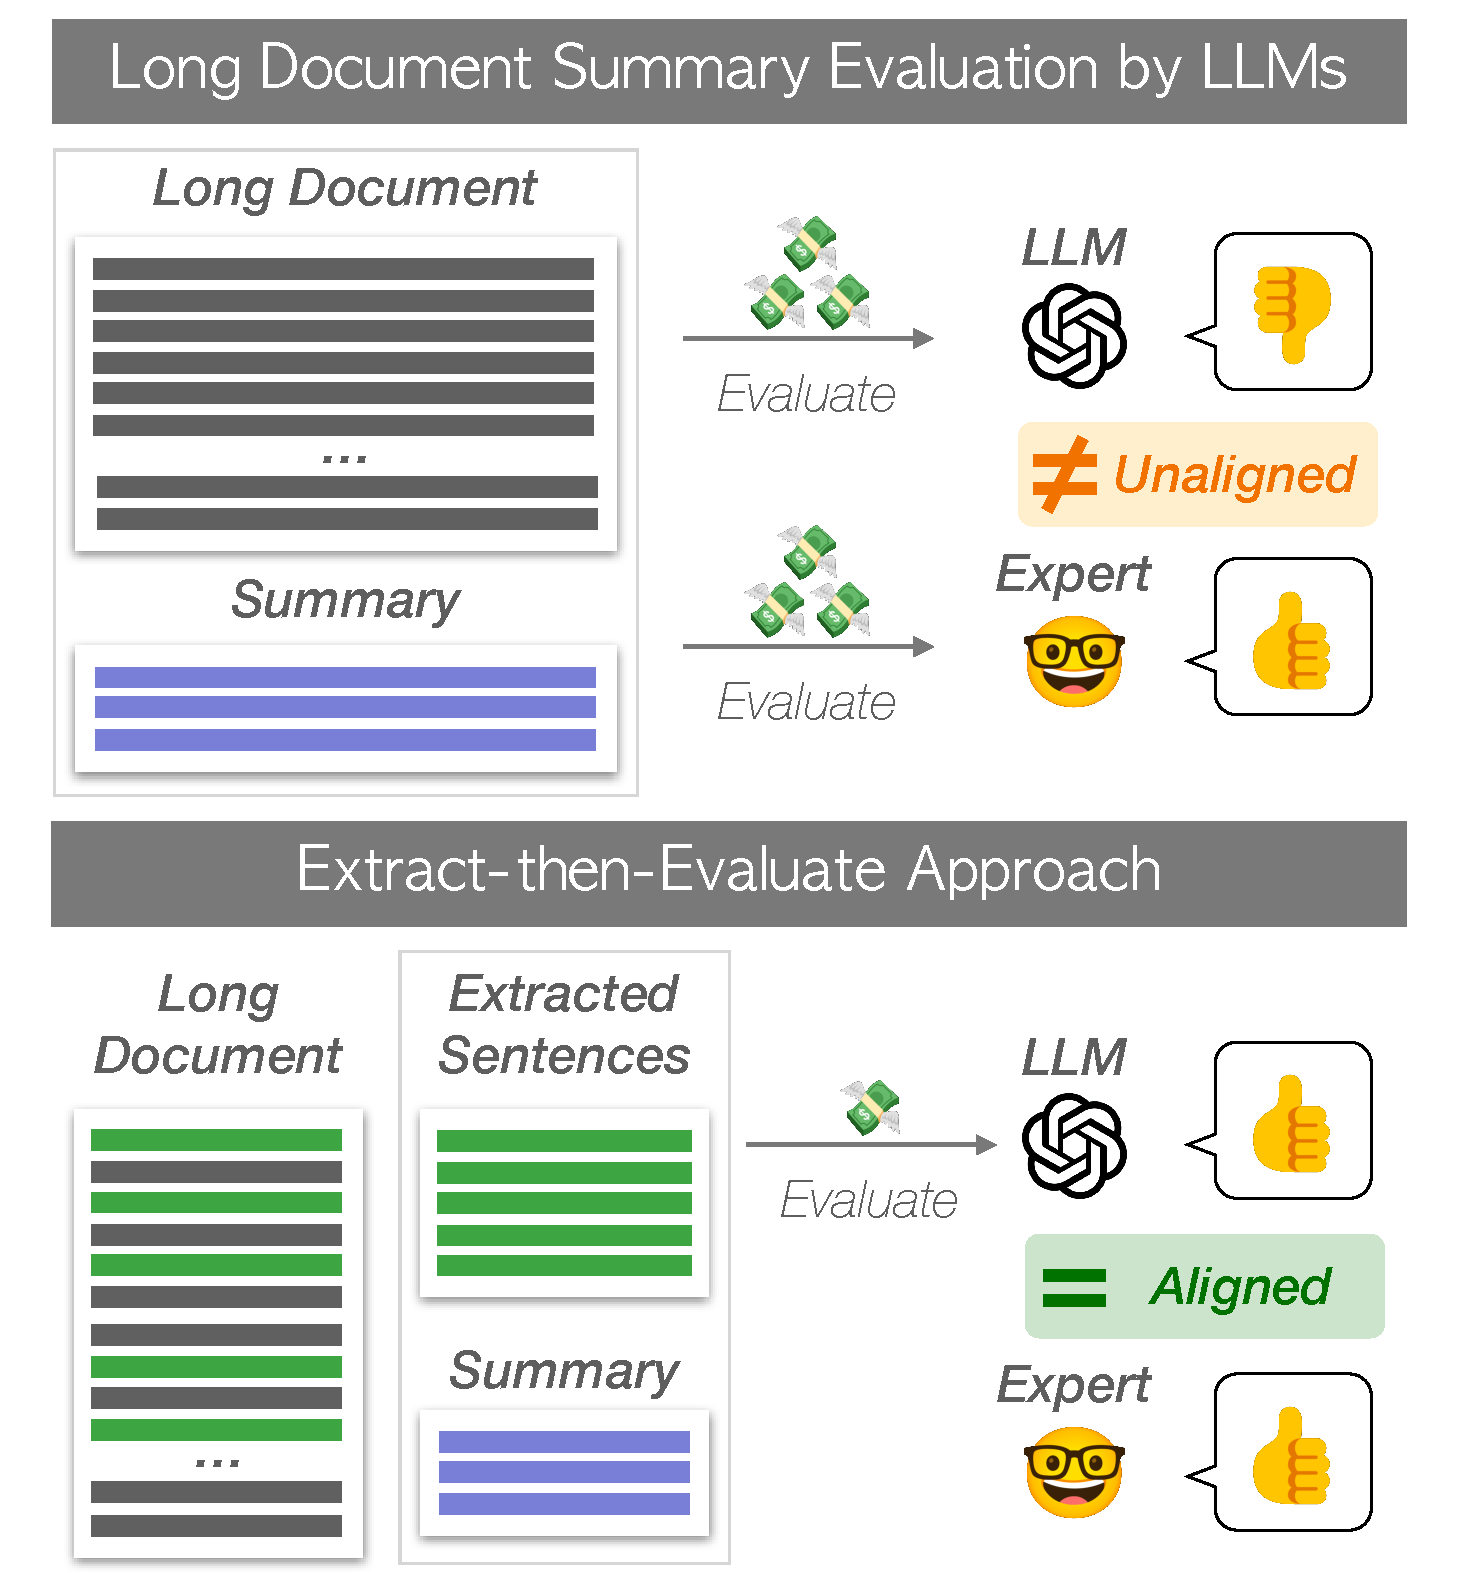
\includegraphics[width=0.5\linewidth]{submissions/Estevam2024/figures/less_is_more.pdf}
  \caption{Overview of the long document summary evaluation task by LLMs. Evaluating long document summaries by LLMs is expensive and shows limited alignment with human evaluations. This study demonstrates that extracting important sentences for evaluation in advance not only reduces evaluation costs but also exhibits better alignment with human evaluations.}
  \label{fig:less_is_more}
\end{figure}

The experiments explore various sentence extraction techniques, encompassing both matching-based and model-based methods, such as LEAD, ROUGE, BERTScore, and NLI. Their performance is evaluated across multiple datasets, including arXiv, GovReport, PubMed, and SQuALITY~\cite{koh-etal-2022-far,krishna-etal-2023-longeval}. The main results are shown in Table~\ref{tab:less_is_more_main_result}. In the experiments, LLMs demonstrated a notable enhancement in correlation with human judgment when compared to non-LLM baselines. However, this improvement came with increased evaluation costs due to the full document prompt length. Extracting key information before evaluation not only reduced costs but also improved performance, attributed to the Lost-in-the-middle problem, where LLMs struggle with critical information in lengthy documents. This trend showed that LLMs perform better with shorter, more informative documents. Lastly, even within a limited budget, the approach delivered comparable performance to top configurations, achieving similar results to the best extraction method while cutting evaluation costs in half.

Based on these observations, it is possible to conclude that effective data pre-processing can reduce costs while allowing the model to concentrate on key information, ultimately enhancing performance.

\begin{table*}[th!]
    \centering
    \small
    \resizebox{\textwidth}{!}{
    \begin{tabular}{lcccccccccccccccccc}
        \toprule
        & \multicolumn{6}{c}{\textbf{Consistency}} & \multicolumn{6}{c}{\textbf{Relevance}} & \multicolumn{6}{c}{\textbf{Faithfulness}}\\
        & \multicolumn{3}{c}{\textbf{arXiv}} & \multicolumn{3}{c}{\textbf{GovReport}} & \multicolumn{3}{c}{\textbf{arXiv}} & \multicolumn{3}{c}{\textbf{GovReport}} & \multicolumn{3}{c}{\textbf{PubMed}} & \multicolumn{3}{c}{\textbf{SQuALITY}} \\
        \cmidrule(lr){2-4} \cmidrule(lr){5-7} \cmidrule(lr){8-10} \cmidrule(lr){11-13} \cmidrule(lr){14-16} \cmidrule(lr){17-19} 
        \textbf{Methods} & $r$ & $\rho$ & $\pounds$ & $r$ & $\rho$ & $\pounds$ & $r$ & $\rho$ & $\pounds$ & $r$ & $\rho$ & $\pounds$ & $r$ & $\rho$ & $\pounds$ & $r$ & $\rho$ & $\pounds$ \\\midrule
        \multicolumn{19}{c}{\textit{Reference-based metrics}}\\
        \midrule
        ROUGE-1 & -0.08 & -0.13 & - & -0.12 & -0.11 & - & 0.29 & 0.25 & - & 0.53 & 0.52 & - & 0.32 & 0.30 & - & -0.33 & -0.13 & -\\
        BERTScore & -0.09 & -0.10 & - & 0.00 & -0.04 & - & 0.22 & 0.18 & - & 0.38 & 0.38 & - & 0.49 & 0.49 & - & -0.12 & 0.02 & -\\
        BARTScore & 0.32 & 0.36 & - & 0.51 & 0.48 & - & 0.00 & 0.03 & - & 0.18 & 0.24 & - & 0.49 & 0.47 & - & -0.06 & -0.17 & -\\
        \midrule
        \multicolumn{19}{c}{\textit{Reference-free metrics}}\\
        \midrule
        FactCC & 0.22 & 0.19 & - & 0.28 & 0.27 & - & 0.13 & 0.13 & - & 0.05 & 0.04 & -  & -0.09 & -0.14 & - & 0.13 & 0.14 & -  \\
        SummaC & 0.32 & 0.32 & - & 0.39 & 0.38 & - & 0.09 & 0.08 & - & 0.05 & 0.04 & - & 0.51 & 0.55 & - & 0.18 & 0.24 & -\\
        \midrule
        \multicolumn{19}{c}{\textit{Reference-free metrics with LLM} (ours)}\\
        \midrule
        Full document & 0.61 & 0.46 & \$0.15 & 0.33 & 0.34 & \$0.10 & 0.58 & 0.52 & \$0.15 & 0.12 & 0.11 & \$0.10 & 0.64 & 0.70 & \$0.11 & 0.51 & 0.38 & \$0.14 \\
        Best extraction & 0.71 & 0.50 & \$0.05 & 0.62 & 0.60 & \$0.09 & 0.63 & 0.58 & \$0.07 & 0.36 & 0.40 & \$0.07 & 0.76 & 0.80 & \$0.07 & 0.85 & 0.81 & \$0.04\\
        Pareto efficient & 0.71 & 0.50 & \$0.05 & 0.60 & 0.61 & \$0.05 & 0.55 & 0.48 & \$0.04 & 0.37 & 0.37 & \$0.05 & 0.75 & 0.75 & \$0.05 & 0.85 & 0.81 & \$0.04\\
        \bottomrule
    \end{tabular}}
    \caption{Results for Pearson correlation ($r$), Spearman correlation ($\rho$), and the average evaluation cost per instance ($\pounds$) indicate that extracting important sentences before evaluation (Best extraction) can yield a higher correlation. Even under a limited budget (Pareto efficient), these results show comparable or even higher correlations compared to the full document setting, with lower costs.}
    \label{tab:less_is_more_main_result}
\end{table*}

\subsection{Model-level enhancements}


Despite ongoing advancements in LLM and RAG models and their continual scaling, there appears to be no clear limit to their growth potential. As a result, integrated systems and workflows—often called compound systems or agentic workflows—are emerging. 
These systems combine LLMs with multiple components, including repeated model calls, retrievers, and external tools, through commercial frameworks like LangChain, LlamaIndex, Auto-GPT, and AgentGPT. Such frameworks empower developers to create agents with unique decision-making capabilities, specialized expertise, and integration with proprietary systems or datasets, as well as build diverse applications ranging from customer service chatbots to advanced decision-support systems. We now highlight several research efforts that showcase compound systems designed to address complex NLP tasks and emphasize that the presence of a System 2 type enhances the performance in such complex tasks.  


\subsubsection{Multi-conditional ranking}

Ranking items based on multiple conditions has wide-ranging applications across various fields. In recommendation systems, for example, once top candidates are shortlisted, re-ranking them according to specific conditions—like genre or category—can greatly enhance the user experience. Similarly, in competitive job markets, this approach is essential for matching resumes to job postings, allowing for prioritization by skills, experience, and other relevant factors.  While there has been considerable advancement in ranking extensive document collections given a query \cite{khattab2020colbert,zhuang2023setwise,qin2023large}, the nuanced task of ranking a smaller set of items based on multiple conditions has not been addressed in prior research.


\begin{figure*}[th!]
    \centering
    \begin{subfigure}[b]{0.24\textwidth}
        \centering
        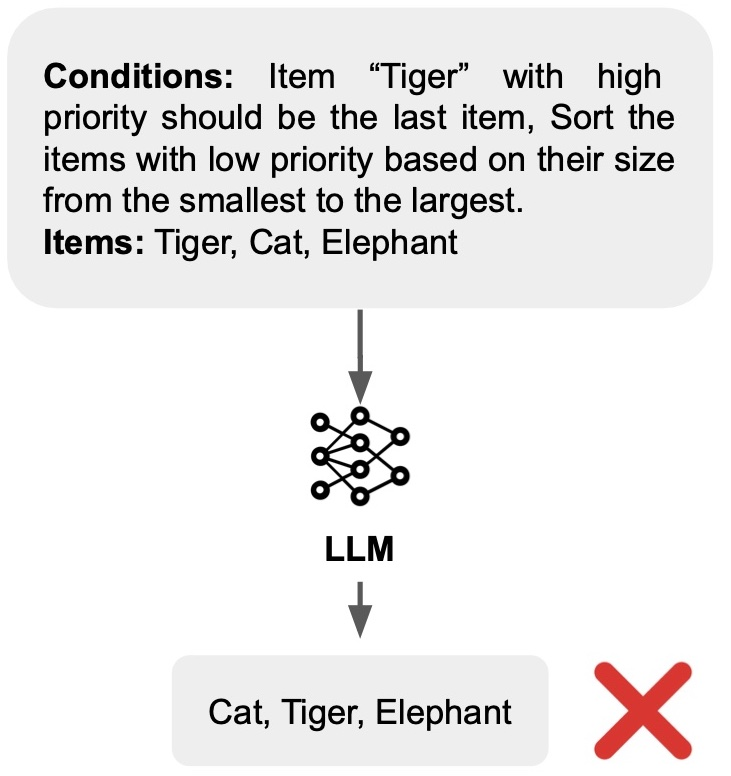
\includegraphics[width=\linewidth]{submissions/Estevam2024/figures/overview-base.jpg}  
        \caption{Base Approach}
    \end{subfigure}%
    ~ 
    \begin{subfigure}[b]{0.65\textwidth}
        \centering
        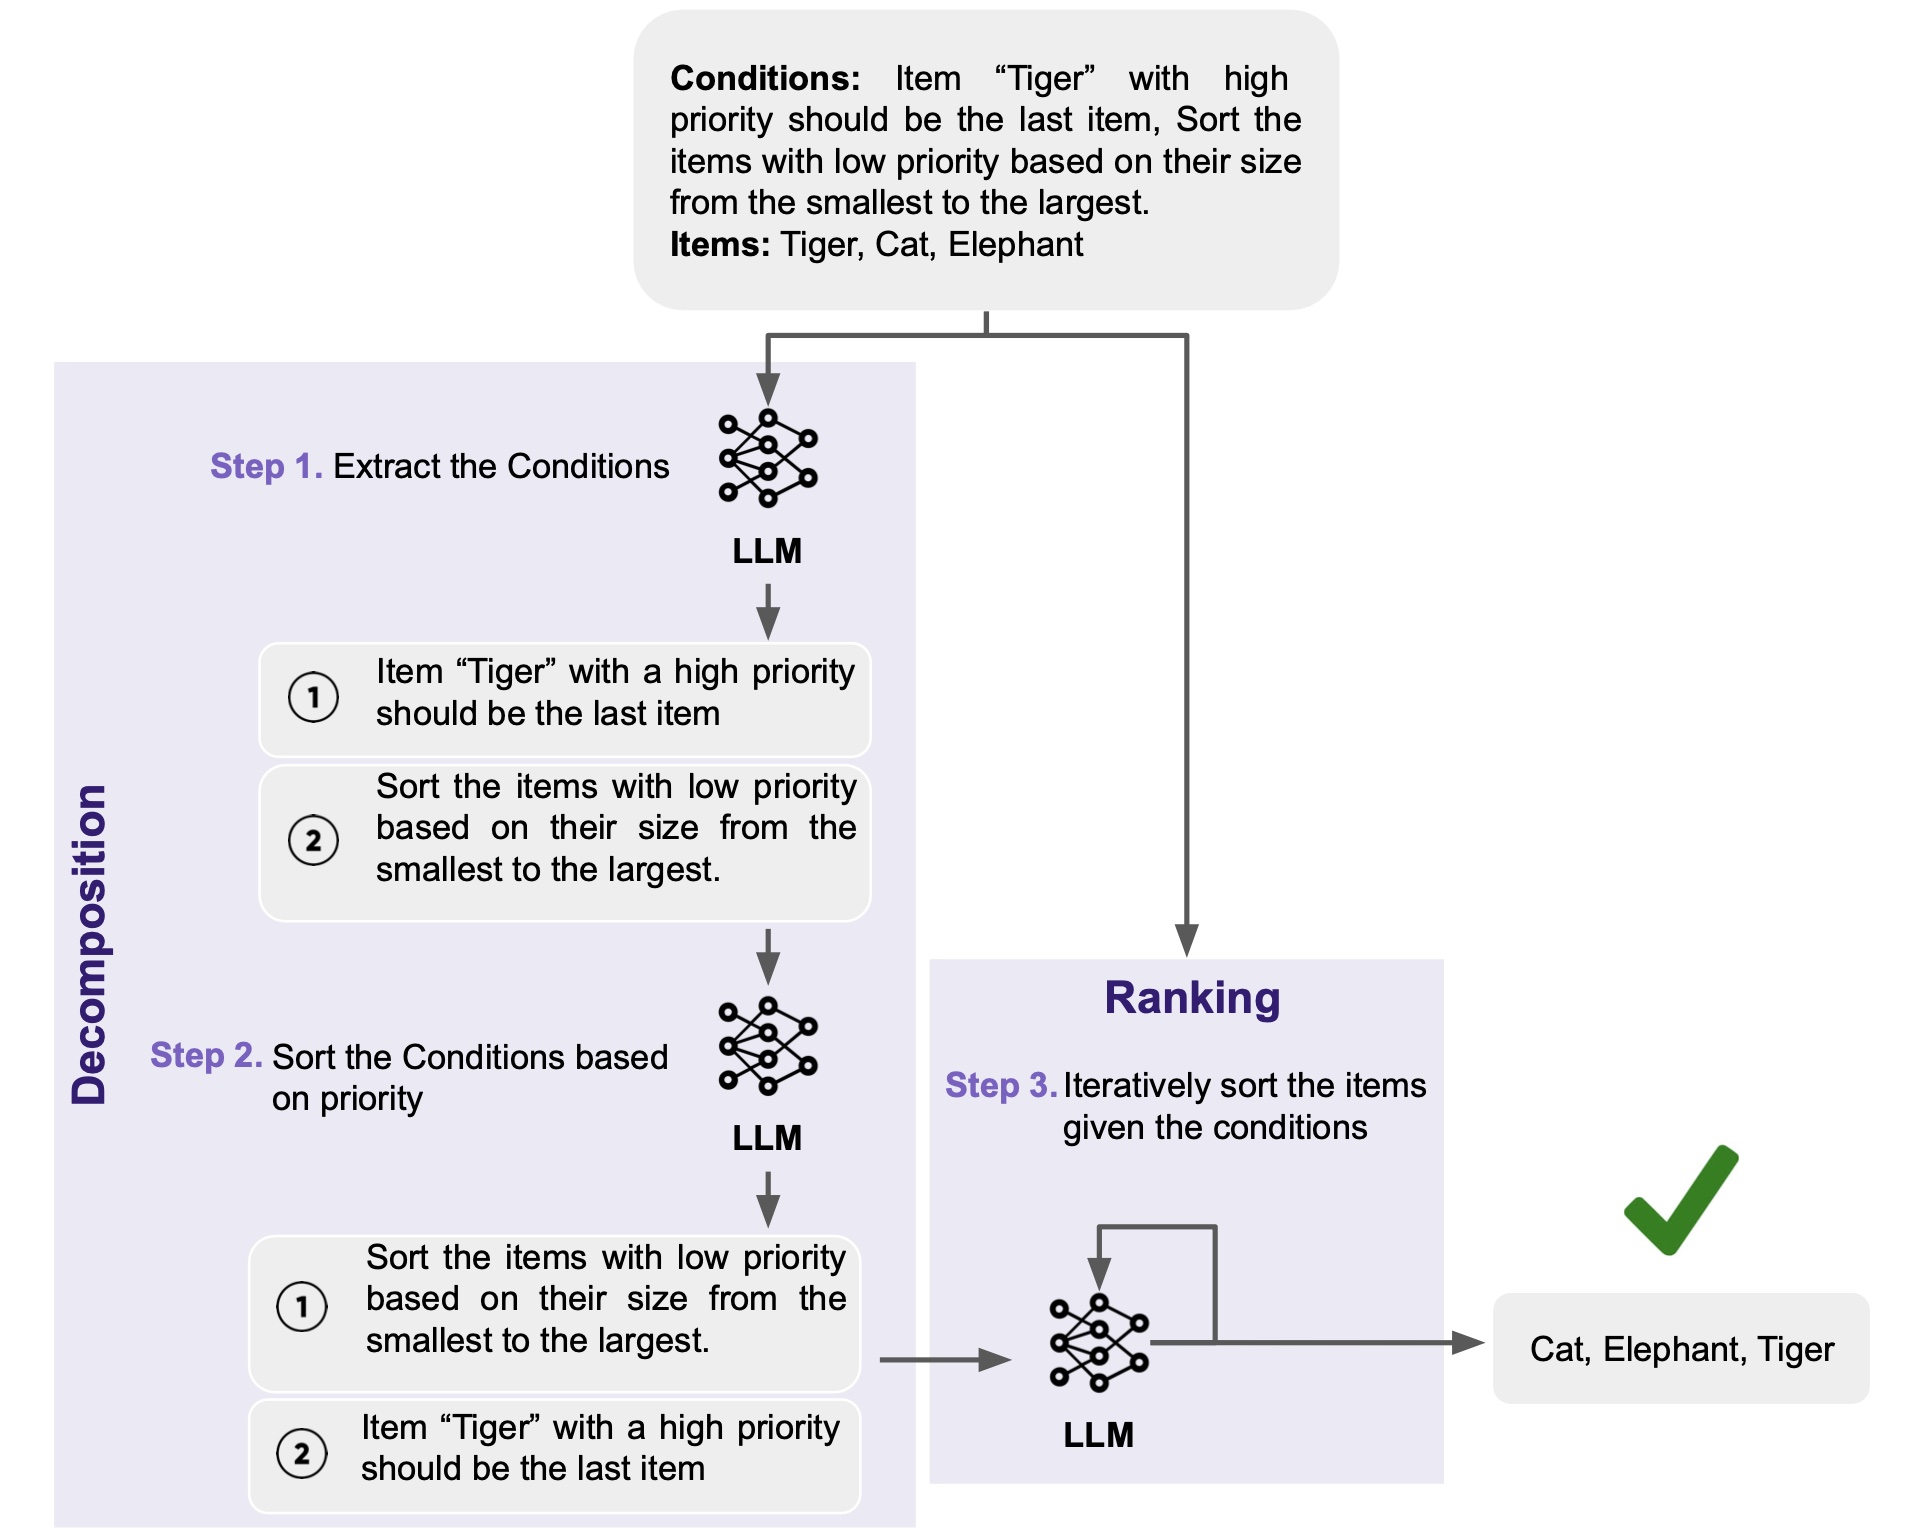
\includegraphics[width=\linewidth]{submissions/Estevam2024/figures/overview-exsir.jpg}
        \caption{EXSIR (Ours)}
    \end{subfigure}  
    \caption{Overview of multi-conditional ranking. Instead of directly prompting LLMs to rank items based on the given conditions, we first extract and sort the conditions based on their priority. Then, we iteratively apply these sorted conditions to the item list.}
    \label{fig:mcr}
\end{figure*}

To address this gap, \cite{pezeshkpour2024multi} defines and investigates the task of multi-conditional ranking (MCR) through the introduction of MCRank, a comprehensive benchmark that encompasses various item types and ranking conditions for evaluating MCR performance. MCRank includes a diverse array of conditions, including positional, locational, temporal, trait-based, and reasoning conditions. Specifically, MCRank was developed by creating a dataset with 18 scenarios varying in item categories, number of conditions (1, 2, or 3), and item set sizes (3, 5, or 7). Each scenario included 200 samples, generated by compiling data and labels for different condition types, featuring randomly ordered item sets with correct rankings. Positional conditions were sourced from Big-Bench's auto-categorization task and Amazon reviews. For scenarios requiring multiple conditions, additional criteria like character counts or positional conditions were added to simulate realistic complexity. This process ensured a robust dataset for evaluating holistic reasoning in scenarios that simulate situations close to real-cases in which users want to rank items based on different conditions defined by their own needs.

Furthermore, we develop EXSIR, a novel decomposed reasoning method that iteratively refines rankings. The process begins with extracting individual conditions from a given string and organizing them into a coherent list. A sorting mechanism then arranges these conditions based on their assigned priorities. Finally, the sorted conditions are applied iteratively to the item list, refining the rankings in each cycle based on the current condition. Figure \ref{fig:mcr} illustrates the workflow of EXSIR along with an example of MCRank.


Initial investigations into existing LLM performance on MCRank show a clear decline in accuracy as both the number of items and conditions increase. Specifically, we observe a sharp drop in ranking accuracy for LLMs like OpenAI o1-mini, GPT-4, ChatGPT (both turbo versions), Llama 3.1-70B, and Mistral (7B) when tasked with three conditions and seven items, with accuracy nearing 0\%.  EXSIR improves ranking accuracy on MCRank by up to 14.4\%, outperforming strong baselines such as Chain-of-Thought (CoT) (see Figure ~\ref{fig:tok-bar}). These results demonstrate how the initial steps towards the System 2 type of thinking (present in the EXSIR approach) allowed to improve the performance of even very strong baselines. 

\begin{figure*}[th!]
    \centering
    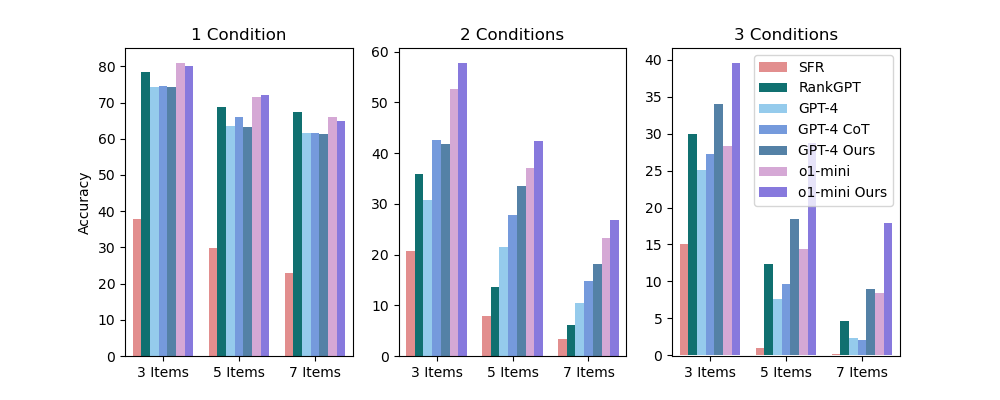
\includegraphics[width=\linewidth]{submissions/Estevam2024/figures/new_token-bar.png}
    \vskip -1.8mm
    \caption{Evaluating the impact of EXSIR against zero-shot CoT prompting for token-level items. We additionally report SFR and RankGPT performances as representatives of existing rankers.}
    \label{fig:tok-bar}
\end{figure*}

\subsubsection{Trust but Verify}
Motivated by the observations from the study reported in Section~\ref{sec:rag_accountable},
we create a two-stage review-then-rationalize (see Figure~\ref{fig:acc-rationalizer}) pipeline to evaluate the impact of intervening  
incorrect model predictions before rationalization. 
The pipeline instruments a \emph{reviewer} module
that employs another LLM (GPT-3.5 \code{text-davinci-003} (\code{temperature = 0})) to evaluate the correctness
of the knowledge-intensive task (KIT) model and refrain from
rationalizing potentially incorrect decisions. 
\begin{figure}[!htb]
    \centering
    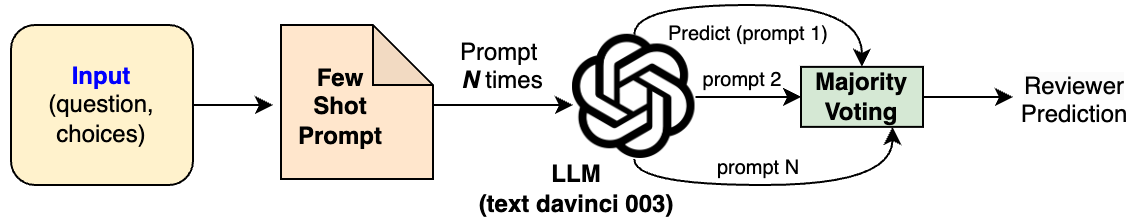
\includegraphics[width=0.7\linewidth]{submissions/Estevam2024/figures/block-accountable.drawio.png}
    \caption{Self-consistency-based Reviewer---intervene for any disagreement with the KIT model prediction.}
    \label{fig:acc-rationalizer}
\end{figure}
 
Depending on the task and data domain, the suitability of the reviewer model may vary. Given the complexity of knowledge-intensive tasks, 
 we employ a self-consistency-based decoding strategy~\cite{wang2022self} where the reviewer is asked the same question $N$ (=5) times, and the final response is selected via majority voting. The reviewer then compares the model's prediction with its prediction, and The rationalizer is utilized only when the KIT model and the reviewer agree. 

 \begin{table}[!htb]
\scriptsize
\centering
\begin{tabular}{cccc}
\hline
\multicolumn{1}{c}{\multirow{2}{*}{\textbf{Dataset}}} & \multicolumn{1}{c}{\textbf{Prediction Errors}} & \multicolumn{2}{c}{\textbf{Errors Intervened}}                                                \\ \cline{3-4} 
\multicolumn{1}{c}{}                                  & \multicolumn{1}{c}{\textbf{(Test Set)}}        & \multicolumn{1}{c}{\textbf{Greedy Decoding}} & \multicolumn{1}{c}{\textbf{Self-consistency}} \\ \hline
CSQA                                                    & 321                                             & \multicolumn{1}{c}{166 ($51.71\%$)}                     & 187 ($\mathbf{58.26\%}$)                                        \\ %\hline
OBQA                                                    & 155                                             & \multicolumn{1}{c}{102 ($65.81\%$)}                     & 110 ($\mathbf{70.97\%}$)                                         \\ \hline
\end{tabular}
\caption{The review-then-rationalize pipeline helps intervene in incorrect predictions of a knowledge-intensive task (KIT) model. The self-consistency-based reviewer outperforms the greedy decoding-based reviewer.}
\label{tab:review}
\end{table}

As shown in Table~\ref{tab:review}, for knowledge-intensive tasks such as Commonsense QA and Openbook QA, the proposed pipeline helps intervene up to $58\%$ and $71\%$ of the incorrect predictions. Unsurprisingly, the self-consistency-based reviewer outperforms the greedy decoding-based reviewer. Overall, \emph{the results draw attention to the importance of responsibly communicating LLM-generated rationales to humans and, consequently, instrumenting guardrails as an effective intervention strategy.} 

\subsection{Orchestration Under Real-World Constraints}
\label{sec:blue-orchestration}
In real-world applications, RAG systems must operate under various constraints such as processing time, resource limitations, and compliance requirements. Efficient orchestration of RAG pipelines, involving the coordination of multiple processes (retrieval, generation, and post-processing), can be challenging but offers unique advantages.
%
We propose a blueprint architecture~\cite{kandogan2024blueprint} where the key orchestration concept is ``streams'' to coordinate the flow of data and instructions among components of varying compute requirements.



Key components in the blueprint architecture include (Figure~\ref{fig:architecture}): (1) \emph{agents, agent and data registries} as key touch points and interfaces to seamlessly integrate with existing deployed models, APIs, databases, and services, (2) \emph{streams} to orchestrate data and instructions across components, and (3) \emph{task and data planners} to optimize for cost and quality constraints in task execution and data retrieval.
%
It is designed for seamless integration into existing infrastructure, enabling extensibility, customizability, and reusability through well-defined touchpoints and interfaces. It supports externalized orchestration and flexible task coordination via declarative plans, ensuring observability, controllability, and optimized performance while meeting quality-of-service constraints.



\begin{figure}[!htb] 
  \vspace{-10pt}
  \centering
  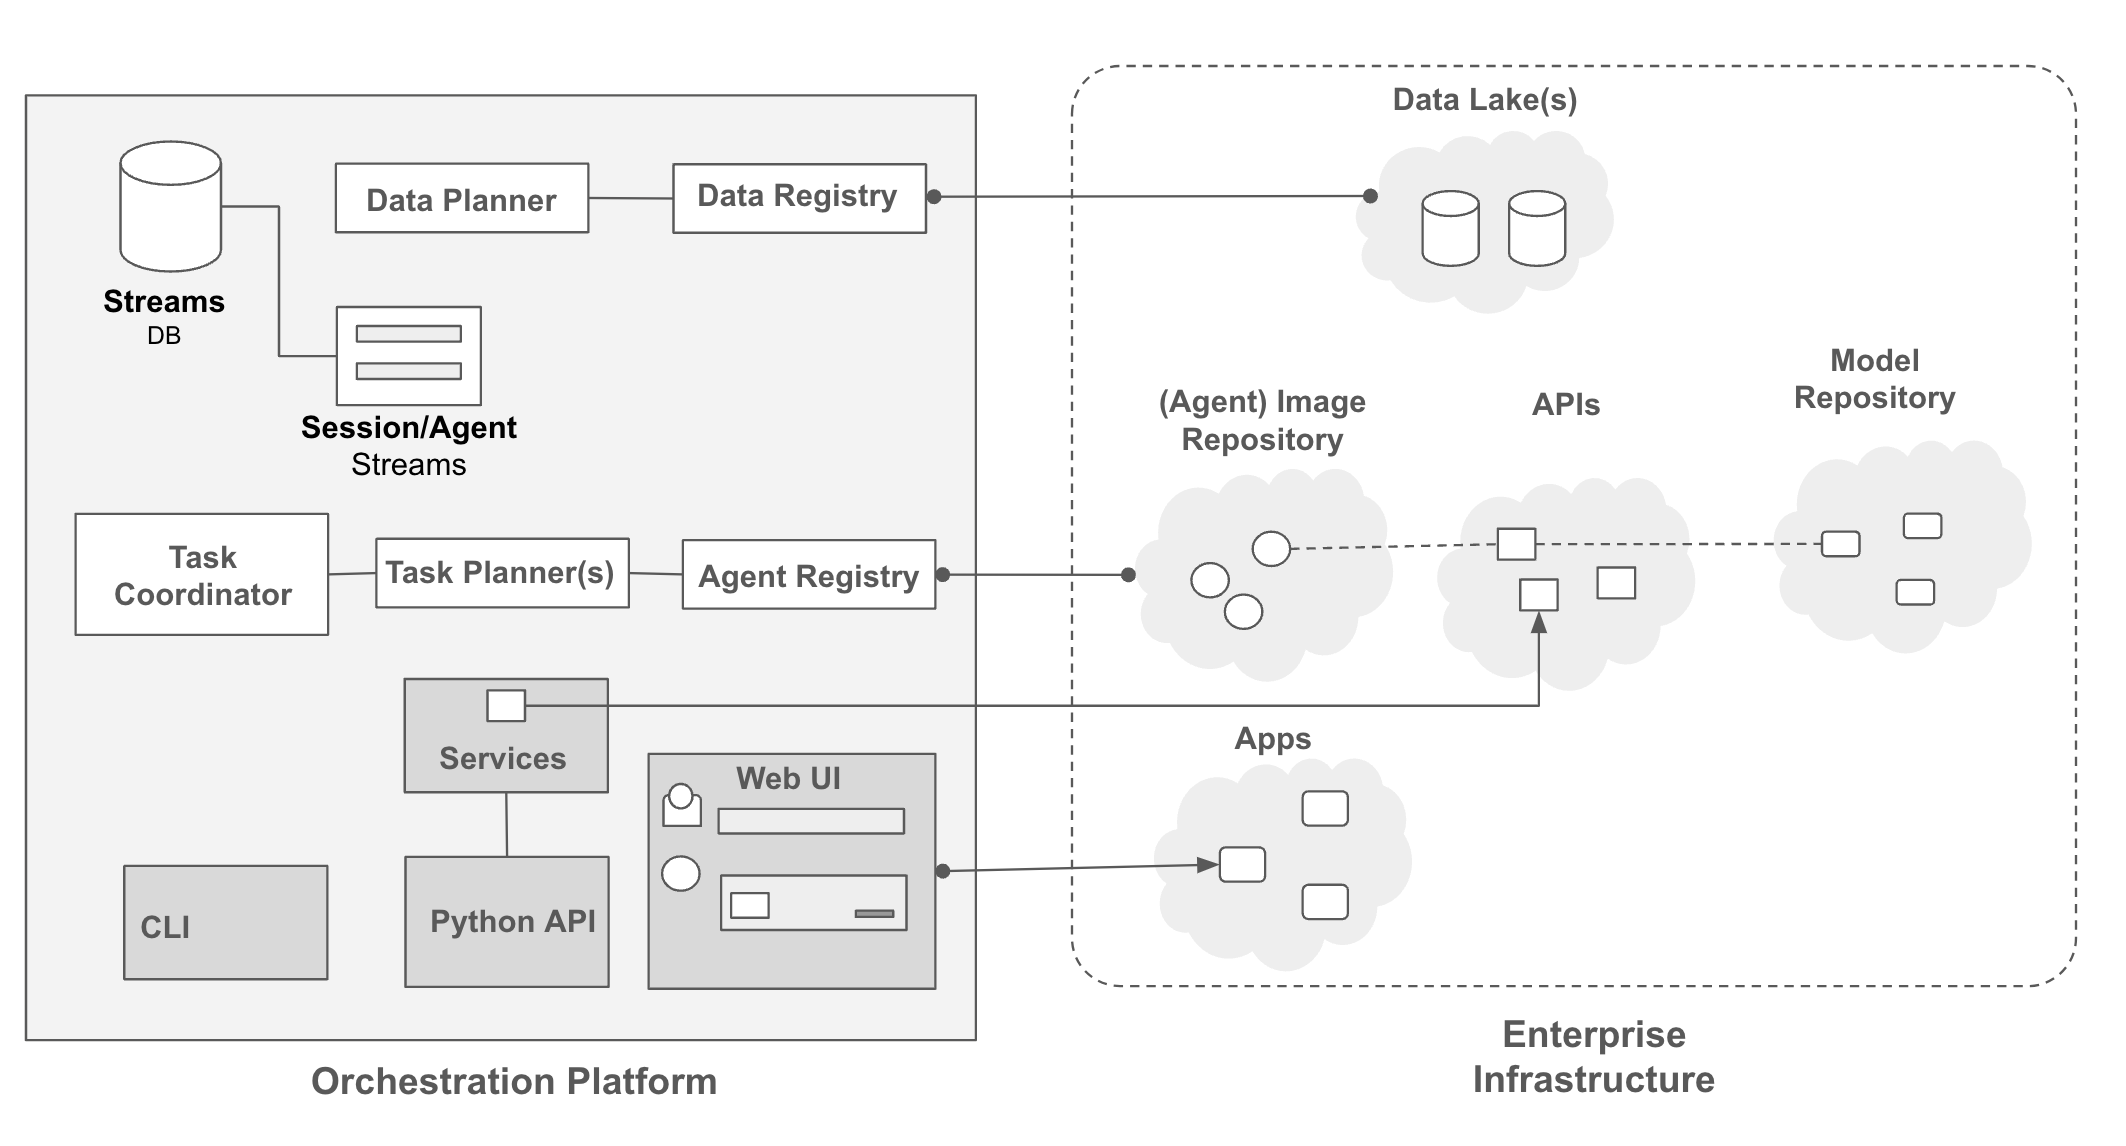
\includegraphics[width=\linewidth]{submissions/Estevam2024/figures/architecture.png}
  \caption{Blueprint Architecture: Data and Agent Registries are touch points that define existing data, models, APIs, and services in the enterprise for utilization by agents.}
  \label{fig:architecture} 
  \vspace{-15pt}
\end{figure}
